\documentclass[14pt,a4paper,oneside]{extreport}
\usepackage[a4paper,top=25mm,bottom=25mm,left=32mm,right=25mm]{geometry}
\usepackage{fontspec,graphicx,longtable,booktabs,array,hyperref,caption,fancyhdr,enumitem,tikz}
\usetikzlibrary{arrows.meta}
\XeTeXlinebreaklocale "th"
\XeTeXlinebreakskip=0pt plus 1pt
\setmainfont{TH Sarabun New}\setsansfont{TH Sarabun New}
\setlength{\parindent}{1.2cm}\setlength{\parskip}{0pt}
\linespread{1.05}
\setlist[enumerate]{leftmargin=1.6cm,itemsep=1pt,topsep=2pt}
\renewcommand{\chaptername}{บทที่}
\renewcommand{\contentsname}{สารบัญ}
\renewcommand{\listtablename}{สารบัญตาราง}
\renewcommand{\listfigurename}{สารบัญภาพ}
\renewcommand{\bibname}{บรรณานุกรม}
\renewcommand{\figurename}{ภาพที่}
\renewcommand{\tablename}{ตารางที่}
\hypersetup{colorlinks=false,pdfborder={0 0 0},pdftitle={รายงานโครงงาน Elegant Solution},pdfauthor={คณะผู้จัดทำโครงงาน}}
\newcolumntype{L}[1]{>{\raggedright\arraybackslash}p{#1}}
\pagestyle{fancy}\fancyhf{}\fancyfoot[C]{\thepage}\renewcommand{\headrulewidth}{0pt}
\captionsetup{font=small,labelfont=bf}
\newcommand{\src}[1]{\par\noindent{\small\textit{ที่มา:} \texttt{\detokenize{#1}}}\par}
\begin{document}
\pagenumbering{gobble}
\begin{titlepage}\centering
\vspace*{23mm}
{\LARGE\bfseries ระบบบริหารจัดการห้องปฏิบัติการและติดตามการใช้คอมพิวเตอร์\par}
\vspace{3mm}{\Large Elegant Solution\par}
\vspace{24mm}
{\Large โดย\par}\vspace{5mm}
{\large ชื่อคนที่ 1\quad รหัสนักศึกษา 0000000001\par}
{\large ชื่อคนที่ 2\quad รหัสนักศึกษา 0000000002\par}
{\large ชื่อคนที่ 3\quad รหัสนักศึกษา 0000000003\par}
\vspace{23mm}{\large อาจารย์ที่ปรึกษา [ระบุชื่ออาจารย์]\par}
\vfill
{\large รายงานวิชาโครงงานเทคโนโลยีสารสนเทศ\par}
{\large หลักสูตรวิทยาศาสตรบัณฑิต\par}
{\large ภาควิชาเทคโนโลยีสารสนเทศ คณะเทคโนโลยีสารสนเทศและนวัตกรรม\par}
{\large มหาวิทยาลัยกรุงเทพ\par}
{\large ภาคการศึกษาที่ [ระบุ] ปีการศึกษา [ระบุ]\par}
\end{titlepage}
\clearpage
\pagenumbering{roman}
\chapter*{บทคัดย่อ}\addcontentsline{toc}{chapter}{บทคัดย่อ}
โครงงาน Elegant Solution พัฒนาระบบบริหารจัดการห้องปฏิบัติการที่เชื่อมข้อมูลผู้ใช้ ตารางเรียน การค้นหาห้อง การจอง และการตรวจสิทธิ์เข้าใช้เข้าด้วยกัน ผู้ดูแลสามารถจัดการห้องและช่วงเวลาที่เปิดใช้งาน พิจารณาคำขอจอง ตรวจประวัติ และติดตามสถานะคอมพิวเตอร์ภายในห้องผ่านเว็บแอปพลิเคชัน ผู้ใช้สามารถค้นหาห้องตามเงื่อนไขและตรวจสถานะการจองของตนเองได้

ระบบประกอบด้วยเว็บแอปพลิเคชันที่พัฒนาด้วย Next.js และ TypeScript ฐานข้อมูล PostgreSQL ผ่าน Prisma บริการ Face AI สำหรับลงทะเบียนและเปรียบเทียบใบหน้า และ Tracking Agent สำหรับรายงานสถานะเครื่องและกิจกรรมในช่วงที่มีผู้ใช้เข้าสู่ Agent session การตรวจสิทธิ์ห้องอาศัยตารางเรียนหรือการจองที่อนุมัติแล้วตามช่วงเวลา โดยบันทึกผลการเข้าใช้และเหตุการณ์ที่เกี่ยวข้องในระบบ

ผลตรวจในสภาพแวดล้อมพัฒนาล่าสุดเมื่อวันที่ 20 พฤศจิกายน 2026 พบว่าชุดทดสอบเว็บแบบไม่ใช้ฐานข้อมูลผ่าน 549 กรณีจาก 25 ไฟล์ รายงานฉบับนี้ใช้ผลดังกล่าวร่วมกับการตรวจซอร์สโค้ดและภาพหน้าจอที่บันทึกจากเว็บจริง โดยแยกการตรวจอัตโนมัติออกจากการพิสูจน์บนอุปกรณ์จริงอย่างชัดเจน

\noindent\textbf{คำสำคัญ:} ห้องปฏิบัติการ การจองห้อง การยืนยันใบหน้า การติดตามคอมพิวเตอร์

\chapter*{ABSTRACT}\addcontentsline{toc}{chapter}{ABSTRACT}
Elegant Solution is a laboratory room management system that brings together user accounts, class schedules, room discovery, reservations, and time-based access decisions. Administrators manage rooms and bookings, review usage records, and monitor laboratory computers. Students and approved guests can discover and reserve eligible rooms through the web application.

The implementation includes a Next.js and TypeScript web application, a PostgreSQL database modeled with Prisma, a Face AI service, and a cross-platform Tracking Agent. Room entitlement is derived from class schedules and approved bookings. The software records access decisions and sessions. In the latest local run on 20 November 2026, 549 web unit tests across 25 files passed.

\noindent\textbf{Keywords:} laboratory management, room booking, face recognition, computer tracking

\chapter*{กิตติกรรมประกาศ}\addcontentsline{toc}{chapter}{กิตติกรรมประกาศ}
รายงานโครงงาน Elegant Solution ฉบับนี้จัดทำขึ้นเพื่อรวบรวมแนวคิด การออกแบบ การพัฒนา และผลการตรวจสอบระบบบริหารจัดการห้องปฏิบัติการและการติดตามการใช้คอมพิวเตอร์ คณะผู้จัดทำขอขอบพระคุณอาจารย์ที่ปรึกษาโครงงาน [ระบุชื่ออาจารย์] สำหรับคำแนะนำในการกำหนดขอบเขตและการเรียบเรียงผลการดำเนินงานให้เป็นรายงานที่ชัดเจน

คณะผู้จัดทำขอขอบคุณคณาจารย์และผู้เกี่ยวข้องกับรายวิชาโครงงานเทคโนโลยีสารสนเทศ ที่สนับสนุนการเรียนรู้และเปิดโอกาสให้พัฒนาโครงงานนี้ รวมถึงผู้พัฒนาเครื่องมือและเอกสารทางเทคนิคที่ใช้ศึกษาและประกอบการพัฒนาระบบ

คณะผู้จัดทำหวังว่ารายงานฉบับนี้จะเป็นประโยชน์ต่อการศึกษาแนวทางบริหารจัดการห้องปฏิบัติการ และเป็นพื้นฐานสำหรับการพัฒนาระบบให้เหมาะสมกับการใช้งานในบริบทจริงต่อไป

\begin{flushright}คณะผู้จัดทำโครงงาน Elegant Solution\end{flushright}

\tableofcontents\clearpage
\phantomsection\addcontentsline{toc}{chapter}{สารบัญตาราง}
\listoftables\clearpage
\phantomsection\addcontentsline{toc}{chapter}{สารบัญภาพ}
\listoffigures\clearpage
\pagenumbering{arabic}
\chapter{บทนำ}
\section{ความเป็นมาของโครงงาน}
การใช้ห้องปฏิบัติการต้องอาศัยข้อมูลหลายส่วนที่เกี่ยวข้องกัน ได้แก่ ผู้ใช้ ห้อง ตารางเรียน ช่วงเวลาว่าง การจอง และสถานะเครื่องคอมพิวเตอร์ หากข้อมูลเหล่านี้แยกกัน ผู้ดูแลต้องตรวจสอบสิทธิ์และการใช้งานจากหลายแหล่ง Elegant Solution จึงออกแบบให้การจัดการห้องและการตัดสินสิทธิ์อยู่บนข้อมูลชุดเดียวกัน พร้อมแสดงผลผ่านเว็บสำหรับผู้ใช้และผู้ดูแล

ในมุมของผู้ใช้ การทราบว่าห้องใดว่างอย่างเดียวไม่เพียงพอต่อการเข้าใช้ห้อง เพราะยังต้องพิจารณาว่าห้องนั้นเปิดให้จองหรือไม่ รองรับกิจกรรมที่ต้องการหรือไม่ และผู้ใช้มีสิทธิ์ในช่วงเวลานั้นจากตารางเรียนหรือคำขอจองที่ได้รับอนุมัติแล้วหรือไม่ ข้อมูลเดียวกันยังเกี่ยวข้องกับจุดตรวจหน้าห้องและการเข้าสู่ระบบของคอมพิวเตอร์ในห้องปฏิบัติการ หากแต่ละส่วนใช้เงื่อนไขต่างกัน ผู้ใช้อาจได้รับผลการตรวจที่ไม่สอดคล้องกัน

โครงงานนี้จึงพัฒนาเว็บแอปพลิเคชันเป็นศูนย์กลางของข้อมูลห้องและสิทธิ์การใช้ห้อง โดยเชื่อมการค้นหาและการจองเข้ากับการตรวจสิทธิ์ ณ เวลาที่ใช้งานจริง พร้อมบริการยืนยันใบหน้าและโปรแกรมติดตามสถานะเครื่องคอมพิวเตอร์ ผู้ดูแลสามารถกำหนดข้อมูลห้อง ตรวจคำขอจอง และดูสถานะการใช้งานผ่านระบบเดียวกัน แนวทางนี้ช่วยให้การอธิบายว่าใครใช้ห้องใดได้ในช่วงเวลาใดอ้างอิงข้อมูลที่ตรวจสอบย้อนหลังได้

\section{วัตถุประสงค์ของโครงงาน}
\begin{enumerate}
\item พัฒนาเว็บสำหรับจัดการบัญชี ห้อง ตารางเรียน และการจองห้องปฏิบัติการ
\item ให้ผู้ใช้ค้นหาห้องที่เหมาะสมและตรวจเงื่อนไขการใช้ห้องตามวันและช่วงเวลา
\item ตรวจสิทธิ์เข้าห้องจากตารางเรียนหรือการจองที่ได้รับอนุมัติ
\item สนับสนุนการยืนยันที่จุดตรวจหน้าห้องด้วยใบหน้าหรือรหัส QR ตามช่องทางที่ระบบเปิดใช้
\item แสดงสถานะเครื่องคอมพิวเตอร์และกิจกรรมในช่วง Agent session สำหรับผู้ดูแล
\end{enumerate}

\section{ขอบเขตของโครงงาน}
ระบบแบ่งการทำงานตามบทบาท Guest, Student, Admin และ Super Admin โดยตรวจสิทธิ์ทั้งในหน้าเว็บและฝั่งเซิร์ฟเวอร์ ขอบเขตการพัฒนาครอบคลุมส่วนต่อไปนี้
\begin{enumerate}
\item \textbf{การจัดการผู้ใช้และห้อง} รองรับการสมัครและเข้าสู่ระบบ การอนุมัติบัญชี Guest การกำหนดข้อมูลห้อง ความจุ คุณสมบัติของห้อง และช่วงเวลาที่เปิดให้จอง
\item \textbf{ตารางเรียน การค้นหา และการจอง} นักศึกษาดูตารางเรียน ค้นหาห้องตามเงื่อนไข และสร้างคำขอจองได้ Guest ที่ได้รับอนุมัติใช้เฉพาะห้องที่เปิดให้ Guest ผู้ดูแลพิจารณาคำขอจองตามนโยบายของห้อง
\item \textbf{การตรวจสิทธิ์เข้าใช้ห้อง} ระบบพิจารณาผู้ใช้ ห้อง และเวลาจากตารางเรียนหรือการจองที่อนุมัติ พร้อมช่องทางตรวจที่ Gate ด้วยใบหน้าหรือ QR ตามเงื่อนไขของแต่ละช่องทาง
\item \textbf{การติดตามคอมพิวเตอร์} Tracking Agent รายงานสถานะเครื่องแก่ผู้ดูแล และบันทึกกิจกรรมที่เกี่ยวข้องกับผู้ใช้เฉพาะช่วงที่มี Agent session
\end{enumerate}

\section{ซอฟต์แวร์และฮาร์ดแวร์ที่ใช้พัฒนา}
โครงงานประกอบด้วยเว็บแอปพลิเคชัน บริการประมวลผลใบหน้า และโปรแกรมที่ติดตั้งบนเครื่องห้องปฏิบัติการ เครื่องมือหลักแบ่งได้ดังนี้
\begin{enumerate}
\item \textbf{เว็บแอปพลิเคชันและฐานข้อมูล} ใช้ Next.js 16, React 19 และ TypeScript สำหรับส่วนเว็บ ใช้ Auth.js จัดการการเข้าสู่ระบบ และใช้ Prisma 7 ร่วมกับ PostgreSQL สำหรับเก็บข้อมูลผู้ใช้ ห้อง ตารางเรียน การจอง และประวัติที่เกี่ยวข้อง
\item \textbf{บริการ Face AI} ใช้ Python, FastAPI และ InsightFace สำหรับตรวจภาพใบหน้าและเปรียบเทียบข้อมูลที่ลงทะเบียน โดยเว็บติดต่อบริการนี้ผ่าน API ภายในระบบ
\item \textbf{Tracking Agent และอุปกรณ์} ใช้ Python พัฒนา Agent สำหรับ Windows, macOS และ Ubuntu การทดลองฟังก์ชันยืนยันใบหน้าต้องมีกล้องและเครื่องที่เปิดเว็บได้ ส่วนการติดตามสถานะต้องติดตั้ง Agent บนคอมพิวเตอร์ห้องปฏิบัติการที่เชื่อมต่อเซิร์ฟเวอร์
\end{enumerate}

\section{ประโยชน์ที่ได้รับ}
การรวมข้อมูลไว้ในระบบเดียวทำให้แต่ละบทบาทเข้าถึงข้อมูลที่จำเป็นต่อการใช้และดูแลห้องปฏิบัติการได้ตามสิทธิ์ที่กำหนด ประโยชน์ที่ได้รับจากระบบมีดังนี้
\begin{enumerate}
\item \textbf{สำหรับนักศึกษาและผู้ใช้ที่ได้รับอนุมัติ} สามารถตรวจข้อมูลห้อง ค้นหาช่วงเวลาที่เหมาะสม และติดตามสถานะการจองผ่านเว็บ โดยไม่ต้องตีความสิทธิ์จากตารางเรียนหรือการจองหลายแห่งด้วยตนเอง
\item \textbf{สำหรับผู้ดูแลระบบ} สามารถกำหนดข้อมูลห้อง พิจารณาคำขอจอง ตรวจประวัติ และดูสถานะคอมพิวเตอร์จากหน้าจัดการที่เชื่อมกับข้อมูลในฐานเดียวกัน
\item \textbf{สำหรับการบริหารห้องปฏิบัติการ} การตรวจสิทธิ์ที่สัมพันธ์กับผู้ใช้ ห้อง และเวลาช่วยให้ผลการอนุญาตมีหลักเกณฑ์ชัดเจน ข้อมูลการใช้ห้องและ log รองรับการตรวจสอบย้อนหลังตามบทบาท
\end{enumerate}

\chapter{ทฤษฎีและเทคโนโลยีที่เกี่ยวข้อง}
\section{เว็บแอปพลิเคชันและการจัดการข้อมูล}
Next.js App Router จัดเส้นทางหน้าเว็บและส่วนทำงานบนเซิร์ฟเวอร์ ส่วน Prisma schema กำหนดแบบข้อมูลและความสัมพันธ์ของฐานข้อมูล PostgreSQL โครงงานใช้แนวทางนี้เพื่อให้บทบาทผู้ใช้ ห้อง ตารางเรียน การจอง และ session มีความสัมพันธ์ตรวจสอบได้ (Next.js, 2026; Prisma, 2026)

\section{การตรวจสิทธิ์ตามบริบท}
การเข้าสู่ระบบเว็บตรวจบัญชีและบทบาท ส่วนสิทธิ์ใช้ห้องต้องพิจารณาคน ห้อง และเวลาร่วมกัน นักศึกษาที่มีตารางเรียนหรือเป็นผู้ร่วมจองในคำขอที่อนุมัติแล้วจึงได้รับสิทธิ์ในช่วงที่กำหนด ข้อมูลการจองถูกเก็บพร้อมผู้เข้าร่วม เพื่อให้การตรวจสิทธิ์ไม่ขึ้นกับสมาชิกกลุ่มที่เปลี่ยนภายหลัง

\begin{figure}[htbp]\centering
\begin{tikzpicture}[>=Stealth,thick,font=\small]
\node[draw,rounded corners,align=center,minimum width=36mm,minimum height=11mm,fill=gray!8] (class) at (0,1.1) {ตารางเรียน\\ตามวันและเวลา};
\node[draw,rounded corners,align=center,minimum width=36mm,minimum height=11mm,fill=gray!8] (booking) at (0,-1.1) {การจองที่อนุมัติ\\และรายชื่อผู้ร่วม};
\node[draw,rounded corners,align=center,minimum width=36mm,minimum height=16mm,fill=blue!5] (check) at (5,0) {ตรวจผู้ใช้ ห้อง\\และเวลาปัจจุบัน};
\node[draw,rounded corners,align=center,minimum width=31mm,minimum height=11mm,fill=gray!8] (gate) at (10,1.1) {Face Gate};
\node[draw,rounded corners,align=center,minimum width=31mm,minimum height=11mm,fill=gray!8] (agent) at (10,-1.1) {Agent login};
\draw[->] (class.east) -- (check.north west);
\draw[->] (booking.east) -- (check.south west);
\draw[->] (check.north east) -- (gate.west);
\draw[->] (check.south east) -- (agent.west);
\end{tikzpicture}
\caption{ข้อมูลที่ใช้ตัดสินสิทธิ์ห้องสำหรับ Face Gate และ Agent login}
\end{figure}

\section{การยืนยันใบหน้าและ QR}
บริการ Face AI ตรวจภาพใบหน้าและสร้าง embedding เพื่อเปรียบเทียบกับข้อมูลที่ลงทะเบียนไว้ โค้ดใช้ InsightFace รุ่น buffalo\_l และ cosine similarity การลงทะเบียนและการตรวจที่ Gate เชื่อมกับเว็บผ่าน API ภายใน ส่วน QR เป็น token สำหรับเข้าใช้ตามห้องและช่วงเวลาที่กำหนด (InsightFace, 2026)

\section{การติดตามเครื่องคอมพิวเตอร์}
Tracking Agent มีส่วน machine service สำหรับส่ง heartbeat และส่วน UI สำหรับ session ของผู้ใช้ การแยกสองส่วนนี้ทำให้ผู้ดูแลเห็นว่าเครื่องออนไลน์แม้ยังไม่มีนักศึกษาเข้าสู่ระบบ Agent จะรายงานกิจกรรมหน้าต่างเฉพาะในช่วง session และขึ้นกับสิทธิ์ที่ระบบปฏิบัติการอนุญาต

\chapter{การวิเคราะห์และออกแบบระบบ}
\section{ขั้นตอนในการดำเนินงาน}
โครงงานเริ่มจากวิเคราะห์บทบาทและข้อมูลที่ต้องใช้ในการบริหารห้อง ออกแบบฐานข้อมูลและการตรวจสิทธิ์ พัฒนาเว็บและบริการประกอบ จากนั้นตรวจด้วยชุดทดสอบอัตโนมัติและเตรียมคู่มือสำหรับการติดตั้ง ภาพที่ 3.1 แสดงความสัมพันธ์ของส่วนประกอบหลัก

ผู้ใช้เข้าถึงเว็บผ่าน HTTPS เว็บตรวจบัญชีและสิทธิ์แล้วอ่านเขียนข้อมูลผ่าน PostgreSQL การลงทะเบียนและตรวจใบหน้าส่งคำขอจากเว็บไป Face AI ภายใน ส่วน Agent ใช้ API สำหรับเปิดใช้งานเครื่อง เข้าสู่ session และส่งสถานะให้หน้าผู้ดูแล โครงสร้างนี้แยกข้อมูลประจำเครื่องออกจาก web session ของผู้ใช้

\begin{figure}[htbp]\centering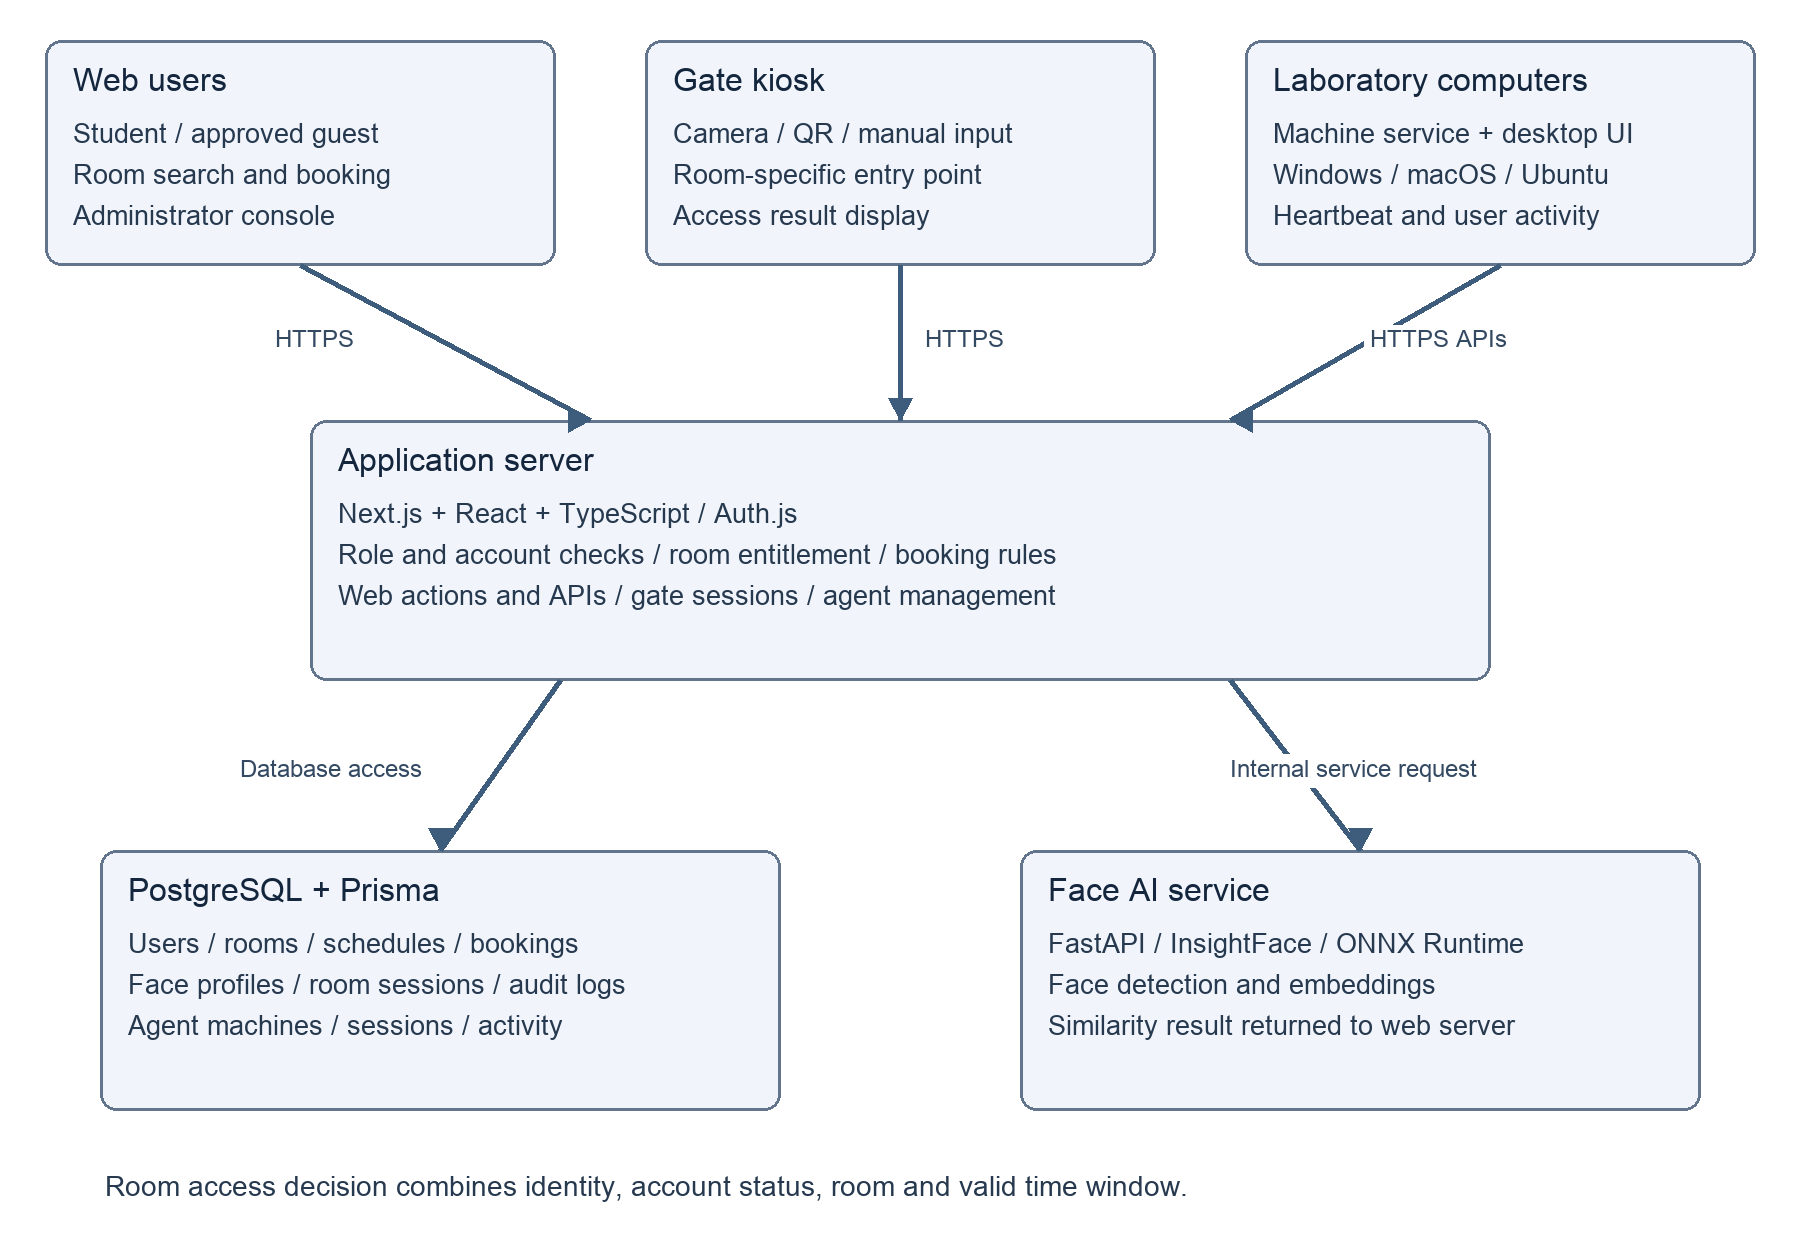
\includegraphics[width=.92\textwidth]{report-assets/architecture.png}\caption{ภาพรวมการทำงานของ Elegant Solution}\end{figure}

\section{พจนานุกรมข้อมูล (Data Dictionary)}
พจนานุกรมข้อมูลต่อไปนี้อ้างอิง \textit{Prisma schema} ของ Elegant Solution โดยคัดฟิลด์สำคัญจากตารางในกระบวนการหลัก ได้แก่ บัญชี ห้อง ตารางเรียน การจอง การยืนยันใบหน้า และการติดตามเครื่อง ชนิดข้อมูลอ้างอิงจาก Prisma โดยใช้คำว่า Enum แทนชนิดที่กำหนดค่าทางเลือกไว้ใน schema เครื่องหมาย ``ไม่'' ในคอลัมน์บังคับหมายถึงฟิลด์ที่อนุญาตค่า \textit{null} ส่วนค่า ``อัตโนมัติ'' หมายถึงมีค่าเริ่มต้นที่ระบบสร้างให้ คอลัมน์คีย์ระบุ PK, FK หรือ UQ (ค่าไม่ซ้ำ)

{\small\setlength{\tabcolsep}{2pt}
\begin{longtable}{L{29mm}L{56mm}L{24mm}L{18mm}L{17mm}}
\caption{ข้อมูลผู้ใช้ (users)}\\\toprule ฟิลด์ & ความหมาย & ชนิด & บังคับ & คีย์\\\midrule\endfirsthead
\toprule ฟิลด์ & ความหมาย & ชนิด & บังคับ & คีย์\\\midrule\endhead
id & รหัสผู้ใช้ที่ระบบสร้าง & String & อัตโนมัติ & PK\\
email & อีเมลสำหรับระบุบัญชี & String & มี & UQ\\
name & ชื่อที่แสดงในระบบ & String & มี & --\\
hashedPassword & ค่ารหัสผ่านที่ผ่านการแฮช & String? & ไม่ & --\\
role & บทบาทผู้ใช้ & Role & อัตโนมัติ & --\\
status & สถานะอนุมัติบัญชี & AccountStatus & อัตโนมัติ & --\\
studentId & รหัสนักศึกษา & String? & ไม่ & UQ\\
createdAt & วันที่สร้างบัญชี & DateTime & อัตโนมัติ & --\\
\bottomrule\end{longtable}

\begin{longtable}{L{29mm}L{56mm}L{24mm}L{18mm}L{17mm}}
\caption{ข้อมูลห้อง (rooms)}\\\toprule ฟิลด์ & ความหมาย & ชนิด & บังคับ & คีย์\\\midrule\endfirsthead
\toprule ฟิลด์ & ความหมาย & ชนิด & บังคับ & คีย์\\\midrule\endhead
id & รหัสห้องที่ระบบสร้าง & String & อัตโนมัติ & PK\\
name & ชื่อห้อง & String & มี & --\\
roomCode & รหัสห้องที่ใช้ค้นหาและอ้างอิง & String & มี & UQ\\
capacity & จำนวนผู้ใช้ที่รองรับ & Int & อัตโนมัติ & --\\
guestAccess & อนุญาต Guest ใช้ห้อง & Boolean & อัตโนมัติ & --\\
isActive & สถานะเปิดใช้ห้อง & Boolean & อัตโนมัติ & --\\
bookingEnabled & เปิดให้จองแบบบริการตนเอง & Boolean & อัตโนมัติ & --\\
approvalPolicy & รูปแบบอนุมัติ AUTO หรือ MANUAL & Enum & อัตโนมัติ & --\\
\bottomrule\end{longtable}

\begin{longtable}{L{29mm}L{56mm}L{24mm}L{18mm}L{17mm}}
\caption{ข้อมูลตารางเรียน (class\_schedules)}\\\toprule ฟิลด์ & ความหมาย & ชนิด & บังคับ & คีย์\\\midrule\endfirsthead
\toprule ฟิลด์ & ความหมาย & ชนิด & บังคับ & คีย์\\\midrule\endhead
id & รหัสรายการตารางเรียน & String & อัตโนมัติ & PK\\
userId & ผู้ใช้เจ้าของตารางเรียน & String & มี & FK users\\
roomId & ห้องเรียน & String & มี & FK rooms\\
dayOfWeek & วันในสัปดาห์ 0 ถึง 6 & Int & มี & --\\
startTime & เวลาเริ่มในรูปแบบ HH:MM & String & มี & --\\
endTime & เวลาสิ้นสุดในรูปแบบ HH:MM & String & มี & --\\
subjectCode & รหัสวิชา & String? & ไม่ & --\\
semester & ภาคการศึกษา & String? & ไม่ & --\\
slot & ช่วงเวลาเรียนตามกริด & AcademicSlot? & ไม่ & --\\
\bottomrule\end{longtable}

\begin{longtable}{L{29mm}L{56mm}L{24mm}L{18mm}L{17mm}}
\caption{ข้อมูลการจองห้อง (room\_bookings)}\\\toprule ฟิลด์ & ความหมาย & ชนิด & บังคับ & คีย์\\\midrule\endfirsthead
\toprule ฟิลด์ & ความหมาย & ชนิด & บังคับ & คีย์\\\midrule\endhead
id & รหัสคำขอจอง & String & อัตโนมัติ & PK\\
roomId & ห้องที่ขอจอง & String & มี & FK rooms\\
userId & ผู้ส่งคำขอจอง & String & มี & FK users\\
date & วันที่จอง (วันตามเวลาไทย) & DateTime & มี & --\\
partySize & จำนวนผู้ใช้ที่คาดว่าจะเข้าห้อง & Int & มี & --\\
purpose & วัตถุประสงค์การจอง & String? & ไม่ & --\\
status & สถานะคำขอจอง & BookingStatus & อัตโนมัติ & --\\
decidedById & ผู้พิจารณาคำขอ & String? & ไม่ & FK users\\
decidedAt & เวลาที่พิจารณา & DateTime? & ไม่ & --\\
\bottomrule\end{longtable}

\begin{longtable}{L{29mm}L{56mm}L{24mm}L{18mm}L{17mm}}
\caption{ช่วงเวลาและผู้เข้าร่วมการจอง}\\\toprule ตารางและฟิลด์ & ความหมาย & ชนิด & บังคับ & คีย์\\\midrule\endfirsthead
\toprule ตารางและฟิลด์ & ความหมาย & ชนิด & บังคับ & คีย์\\\midrule\endhead
slots.id & รหัสช่วงเวลาการจอง & String & อัตโนมัติ & PK\\
slots.bookingId & คำขอจองเจ้าของช่วงเวลา & String & มี & FK bookings\\
slots.slot & ช่วงเวลาเรียนที่จอง & AcademicSlot & มี & --\\
slots.startAt & เวลาเริ่มใช้ห้องจริง & DateTime & มี & --\\
slots.endAt & เวลาสิ้นสุดใช้ห้องจริง & DateTime & มี & --\\
participants.id & รหัสรายการผู้เข้าร่วม & String & อัตโนมัติ & PK\\
participants.bookingId & คำขอจองเจ้าของรายการ & String & มี & FK bookings\\
participants.userId & ผู้มีสิทธิ์ร่วมการจอง & String & มี & FK users\\
participants.source & ที่มาของสิทธิ์ SELF หรือ GROUP & Enum & มี & --\\
\bottomrule\end{longtable}

\begin{longtable}{L{29mm}L{56mm}L{24mm}L{18mm}L{17mm}}
\caption{ข้อมูลใบหน้าและการใช้ห้อง}\\\toprule ตารางและฟิลด์ & ความหมาย & ชนิด & บังคับ & คีย์\\\midrule\endfirsthead
\toprule ตารางและฟิลด์ & ความหมาย & ชนิด & บังคับ & คีย์\\\midrule\endhead
face.id & รหัสโปรไฟล์ใบหน้า & String & อัตโนมัติ & PK\\
face.userId & เจ้าของข้อมูลใบหน้า & String & มี & FK users, UQ\\
face.embedding & เวกเตอร์ลักษณะใบหน้า & Float[] & มี & --\\
face.modelVersion & ชื่อรุ่นโมเดล AI & String & อัตโนมัติ & --\\
session.id & รหัสครั้งที่ใช้ห้อง & String & อัตโนมัติ & PK\\
session.userId & ผู้ใช้ห้อง & String & มี & FK users\\
session.roomId & ห้องที่ใช้ & String & มี & FK rooms\\
session.checkIn & เวลาเข้าใช้ & DateTime & อัตโนมัติ & --\\
session.checkOut & เวลาออกจากห้อง & DateTime? & ไม่ & --\\
\bottomrule\end{longtable}

\clearpage
\begin{longtable}{L{29mm}L{56mm}L{24mm}L{18mm}L{17mm}}
\caption{ข้อมูลเครื่องและ Agent session}\\\toprule ตารางและฟิลด์ & ความหมาย & ชนิด & บังคับ & คีย์\\\midrule\endfirsthead
\toprule ตารางและฟิลด์ & ความหมาย & ชนิด & บังคับ & คีย์\\\midrule\endhead
machine.id & รหัสเครื่อง & String & อัตโนมัติ & PK\\
machine.machineCode & รหัสแสดงเครื่อง & String & มี & UQ\\
machine.roomId & ห้องที่เครื่องสังกัด & String? & ไม่ & FK rooms\\
machine.lastSeen & เวลารับ heartbeat ล่าสุด & DateTime? & ไม่ & --\\
agentSession.id & รหัส Agent session & String & อัตโนมัติ & PK\\
agentSession.userId & ผู้ใช้ที่เข้าสู่เครื่อง & String & มี & FK users\\
agentSession.machineId & เครื่องที่ถูกใช้งาน & String & มี & FK machines\\
agentSession.roomId & ห้องที่สัมพันธ์กับ session & String & มี & FK rooms\\
agentSession.expiresAt & เวลาหมดอายุ session & DateTime & มี & --\\
\bottomrule\end{longtable}
}

ชื่อตารางจริงในฐานข้อมูลใช้รูปพหูพจน์ตามคำสั่ง map ใน schema เช่น users, rooms และ room\_bookings ตาราง RoomBookingSlot และ RoomBookingParticipant ใช้เก็บช่วงเวลาและรายชื่อผู้มีสิทธิ์ที่บันทึก ณ เวลาสร้างการจอง รายละเอียดฟิลด์ทั้งหมดสามารถตรวจได้จาก web/prisma/schema.prisma

\section{บทบาทและกรณีใช้งาน}
\begin{longtable}{L{33mm}L{105mm}}\caption{บทบาทและกรณีใช้งานหลัก}\\\toprule บทบาท & กรณีใช้งานหลัก\\\midrule\endfirsthead
\toprule บทบาท & กรณีใช้งานหลัก\\\midrule\endhead
Guest & สมัครบัญชี รออนุมัติ ค้นหาและจองห้องที่เปิดให้ Guest\\
Student & เข้าสู่ระบบ ตรวจตารางเรียน ค้นหาและจองห้อง ตรวจสิทธิ์เข้าใช้\\
Admin & จัดการผู้ใช้ ห้อง ตารางเรียน การจอง และดูสถานะเครื่อง\\
Super Admin & จัดการระบบและสร้างชุดรหัสเปิดใช้งาน Tracking Agent\\\bottomrule\end{longtable}

\section{แบบจำลองฐานข้อมูล}
Prisma schema ของโครงงานประกอบด้วย User, Room, ClassSchedule, RoomBooking, RoomBookingParticipant, AccessToken, FaceProfile, Session และกลุ่มตาราง Agent ความสัมพันธ์สำคัญคือผู้ใช้จองห้องตาม slot ที่กำหนด การอนุมัติจองทำให้ผู้เข้าร่วมที่บันทึกไว้มีสิทธิ์ตามเวลา และ machine session ผูกเครื่องกับผู้ใช้ที่ผ่านการตรวจบัญชีและสิทธิ์

\begin{longtable}{L{40mm}L{98mm}}\caption{กลุ่มข้อมูลสำคัญในฐานข้อมูล}\\\toprule กลุ่มข้อมูล & หน้าที่\\\midrule\endfirsthead
\toprule กลุ่มข้อมูล & หน้าที่\\\midrule\endhead
User และ FaceProfile & เก็บบัญชี บทบาท สถานะ และข้อมูลสำหรับการเทียบใบหน้า\\
Room และ RoomAvailabilityWindow & กำหนดห้อง ความจุ ความสามารถ และช่วงที่เปิดให้ใช้\\
ClassSchedule และ RoomBooking & เก็บตารางเรียน คำขอจอง slot และผู้เข้าร่วม\\
Session และ Log & บันทึกการใช้ห้องและเหตุการณ์ที่เกี่ยวข้อง\\
AgentMachine และ AgentSession & เก็บสถานะเครื่องและ session ของผู้ใช้เครื่อง\\\bottomrule\end{longtable}

\section{ลำดับการทำงานที่สำคัญ}
ผู้ใช้เข้าสู่ระบบแล้วค้นหาห้อง ระบบตรวจวัน เวลา ความพร้อม และเงื่อนไขของห้อง เมื่อสร้างคำขอจองจะได้สถานะตามนโยบายอนุมัติของห้อง ผู้ใช้ที่มีสิทธิ์ตามตารางเรียนหรือการจองจึงผ่านการตรวจที่จุด Gate ได้ สำหรับเครื่องคอมพิวเตอร์ Agent ยืนยันเครื่องและส่ง heartbeat อย่างต่อเนื่อง ส่วนกิจกรรมผู้ใช้เริ่มหลัง Agent login ที่ผ่านการตรวจสิทธิ์ห้อง

\chapter{ผลการพัฒนาและการตรวจสอบ}
\section{ส่วนของผู้ใช้งาน}
หน้าเว็บจริงแสดงทางเข้าสู่ระบบและข้อมูลห้อง ผู้ใช้ที่มีสิทธิ์สามารถเข้าสู่หน้า Dashboard เพื่อตรวจตารางเรียนและการจอง และค้นหาห้องตามเงื่อนไขที่ต้องการ
\begin{figure}[htbp]\centering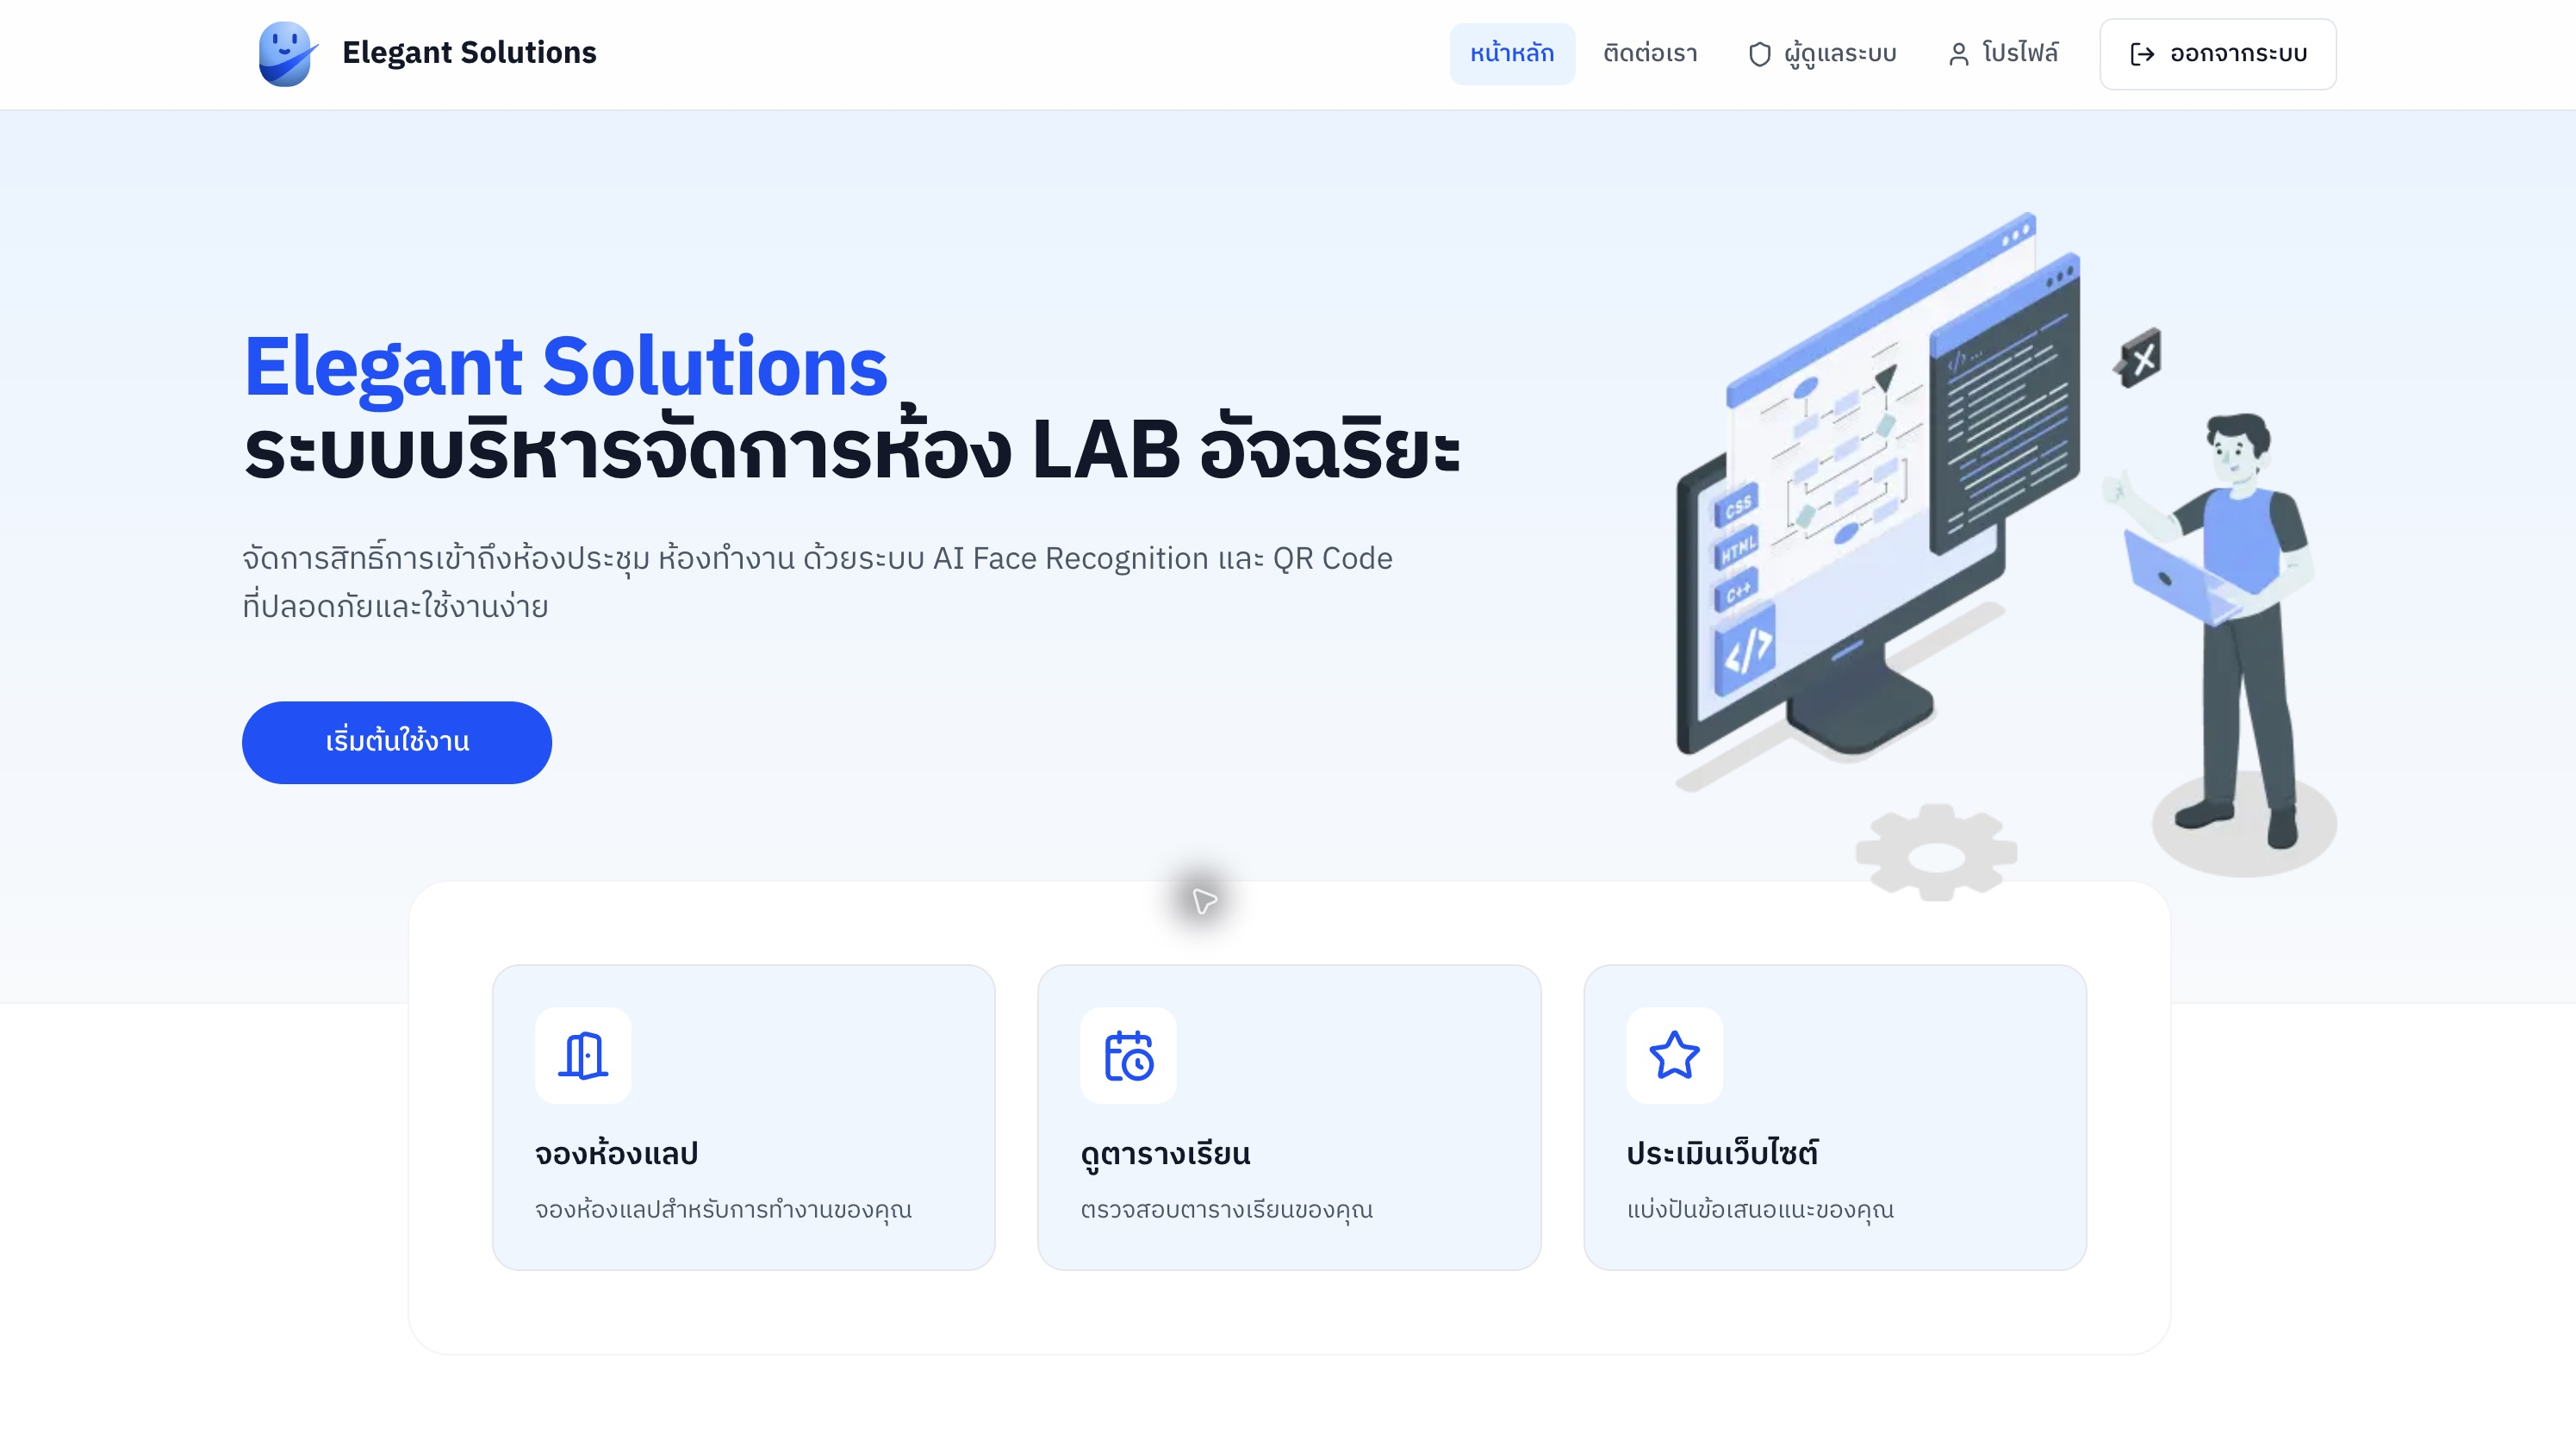
\includegraphics[width=.82\textwidth]{report-assets/ui-home-crop.png}\caption{หน้าเว็บ Elegant Solution}\end{figure}
\begin{figure}[htbp]\centering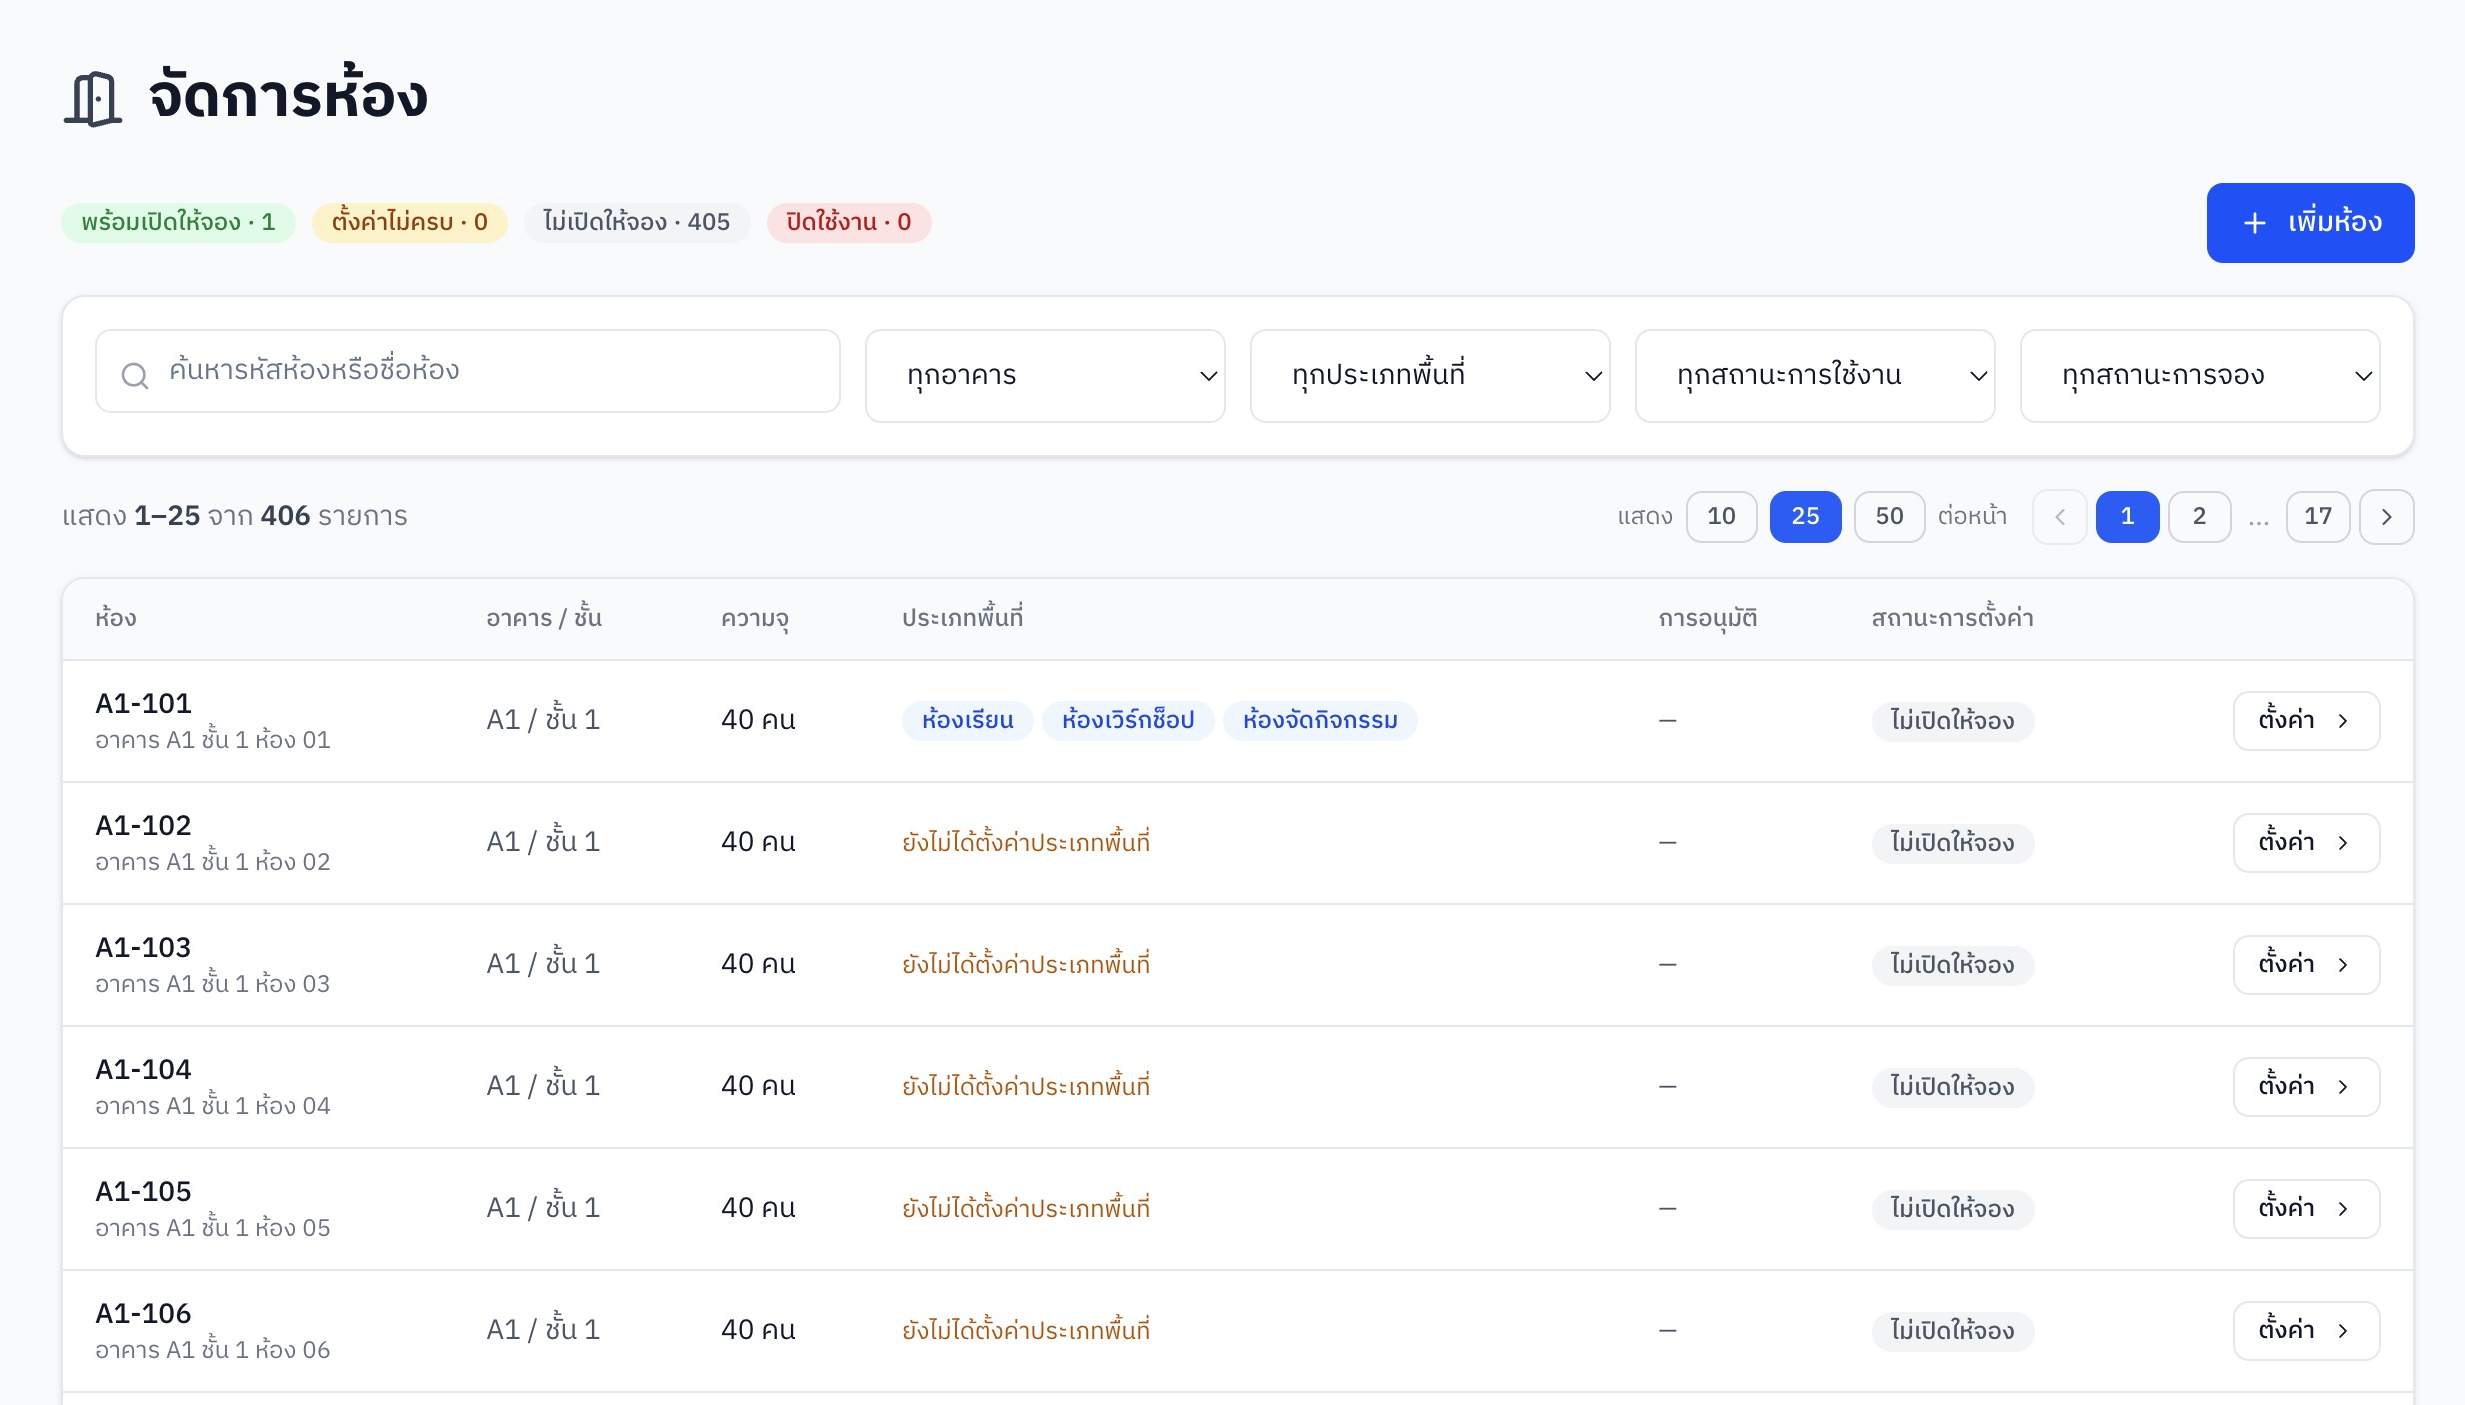
\includegraphics[width=.82\textwidth]{report-assets/ui-rooms-crop.png}\caption{หน้าจัดการห้องในระบบจริง}\end{figure}

\section{ส่วนของผู้ดูแลระบบ}
ผู้ดูแลมีหน้า Dashboard สำหรับดูภาพรวม และหน้าเฉพาะสำหรับจัดการผู้ใช้ ห้อง การจอง ตารางเรียน รายงาน และสถานะเครื่อง การกำหนดสิทธิ์ใน server action และ API เป็นตัวควบคุมการเข้าถึงข้อมูล
\begin{figure}[htbp]\centering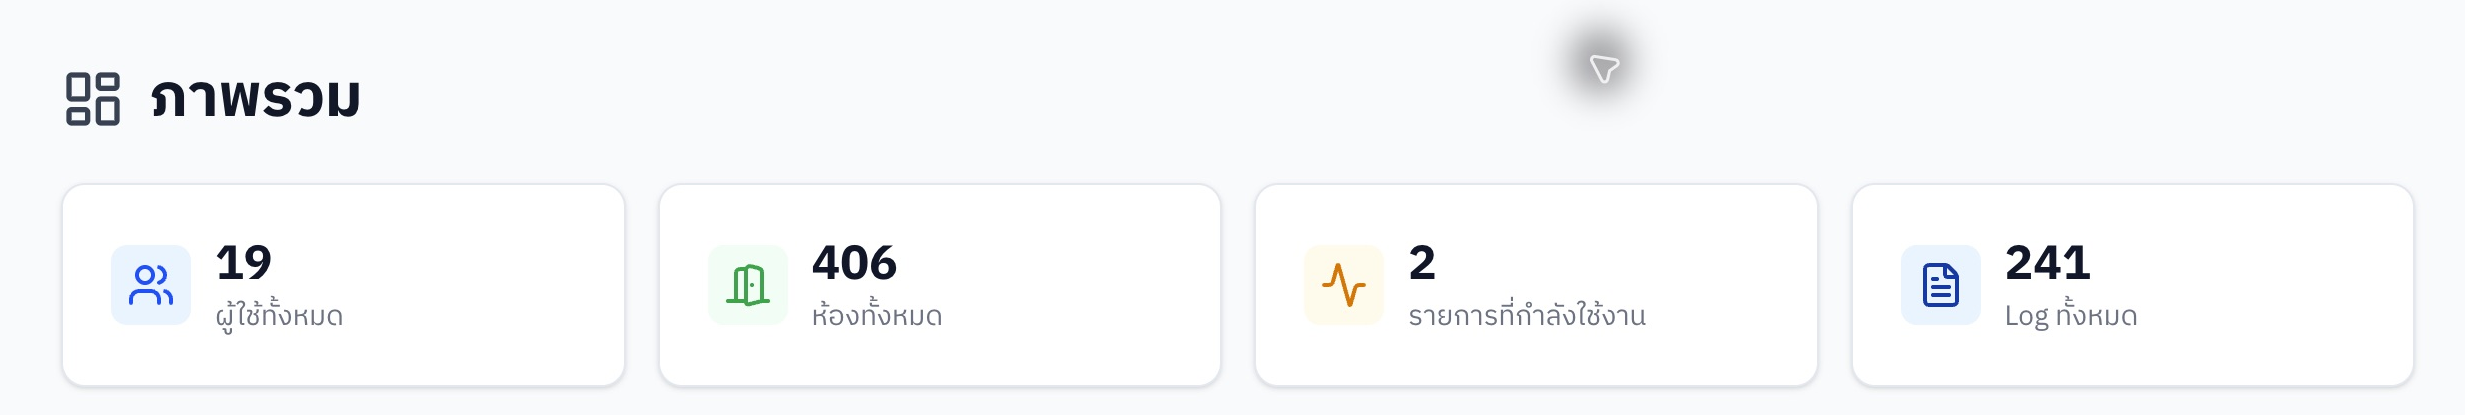
\includegraphics[width=.82\textwidth]{report-assets/ui-admin-crop.png}\caption{หน้าภาพรวมสำหรับผู้ดูแลระบบ}\end{figure}
\begin{figure}[htbp]\centering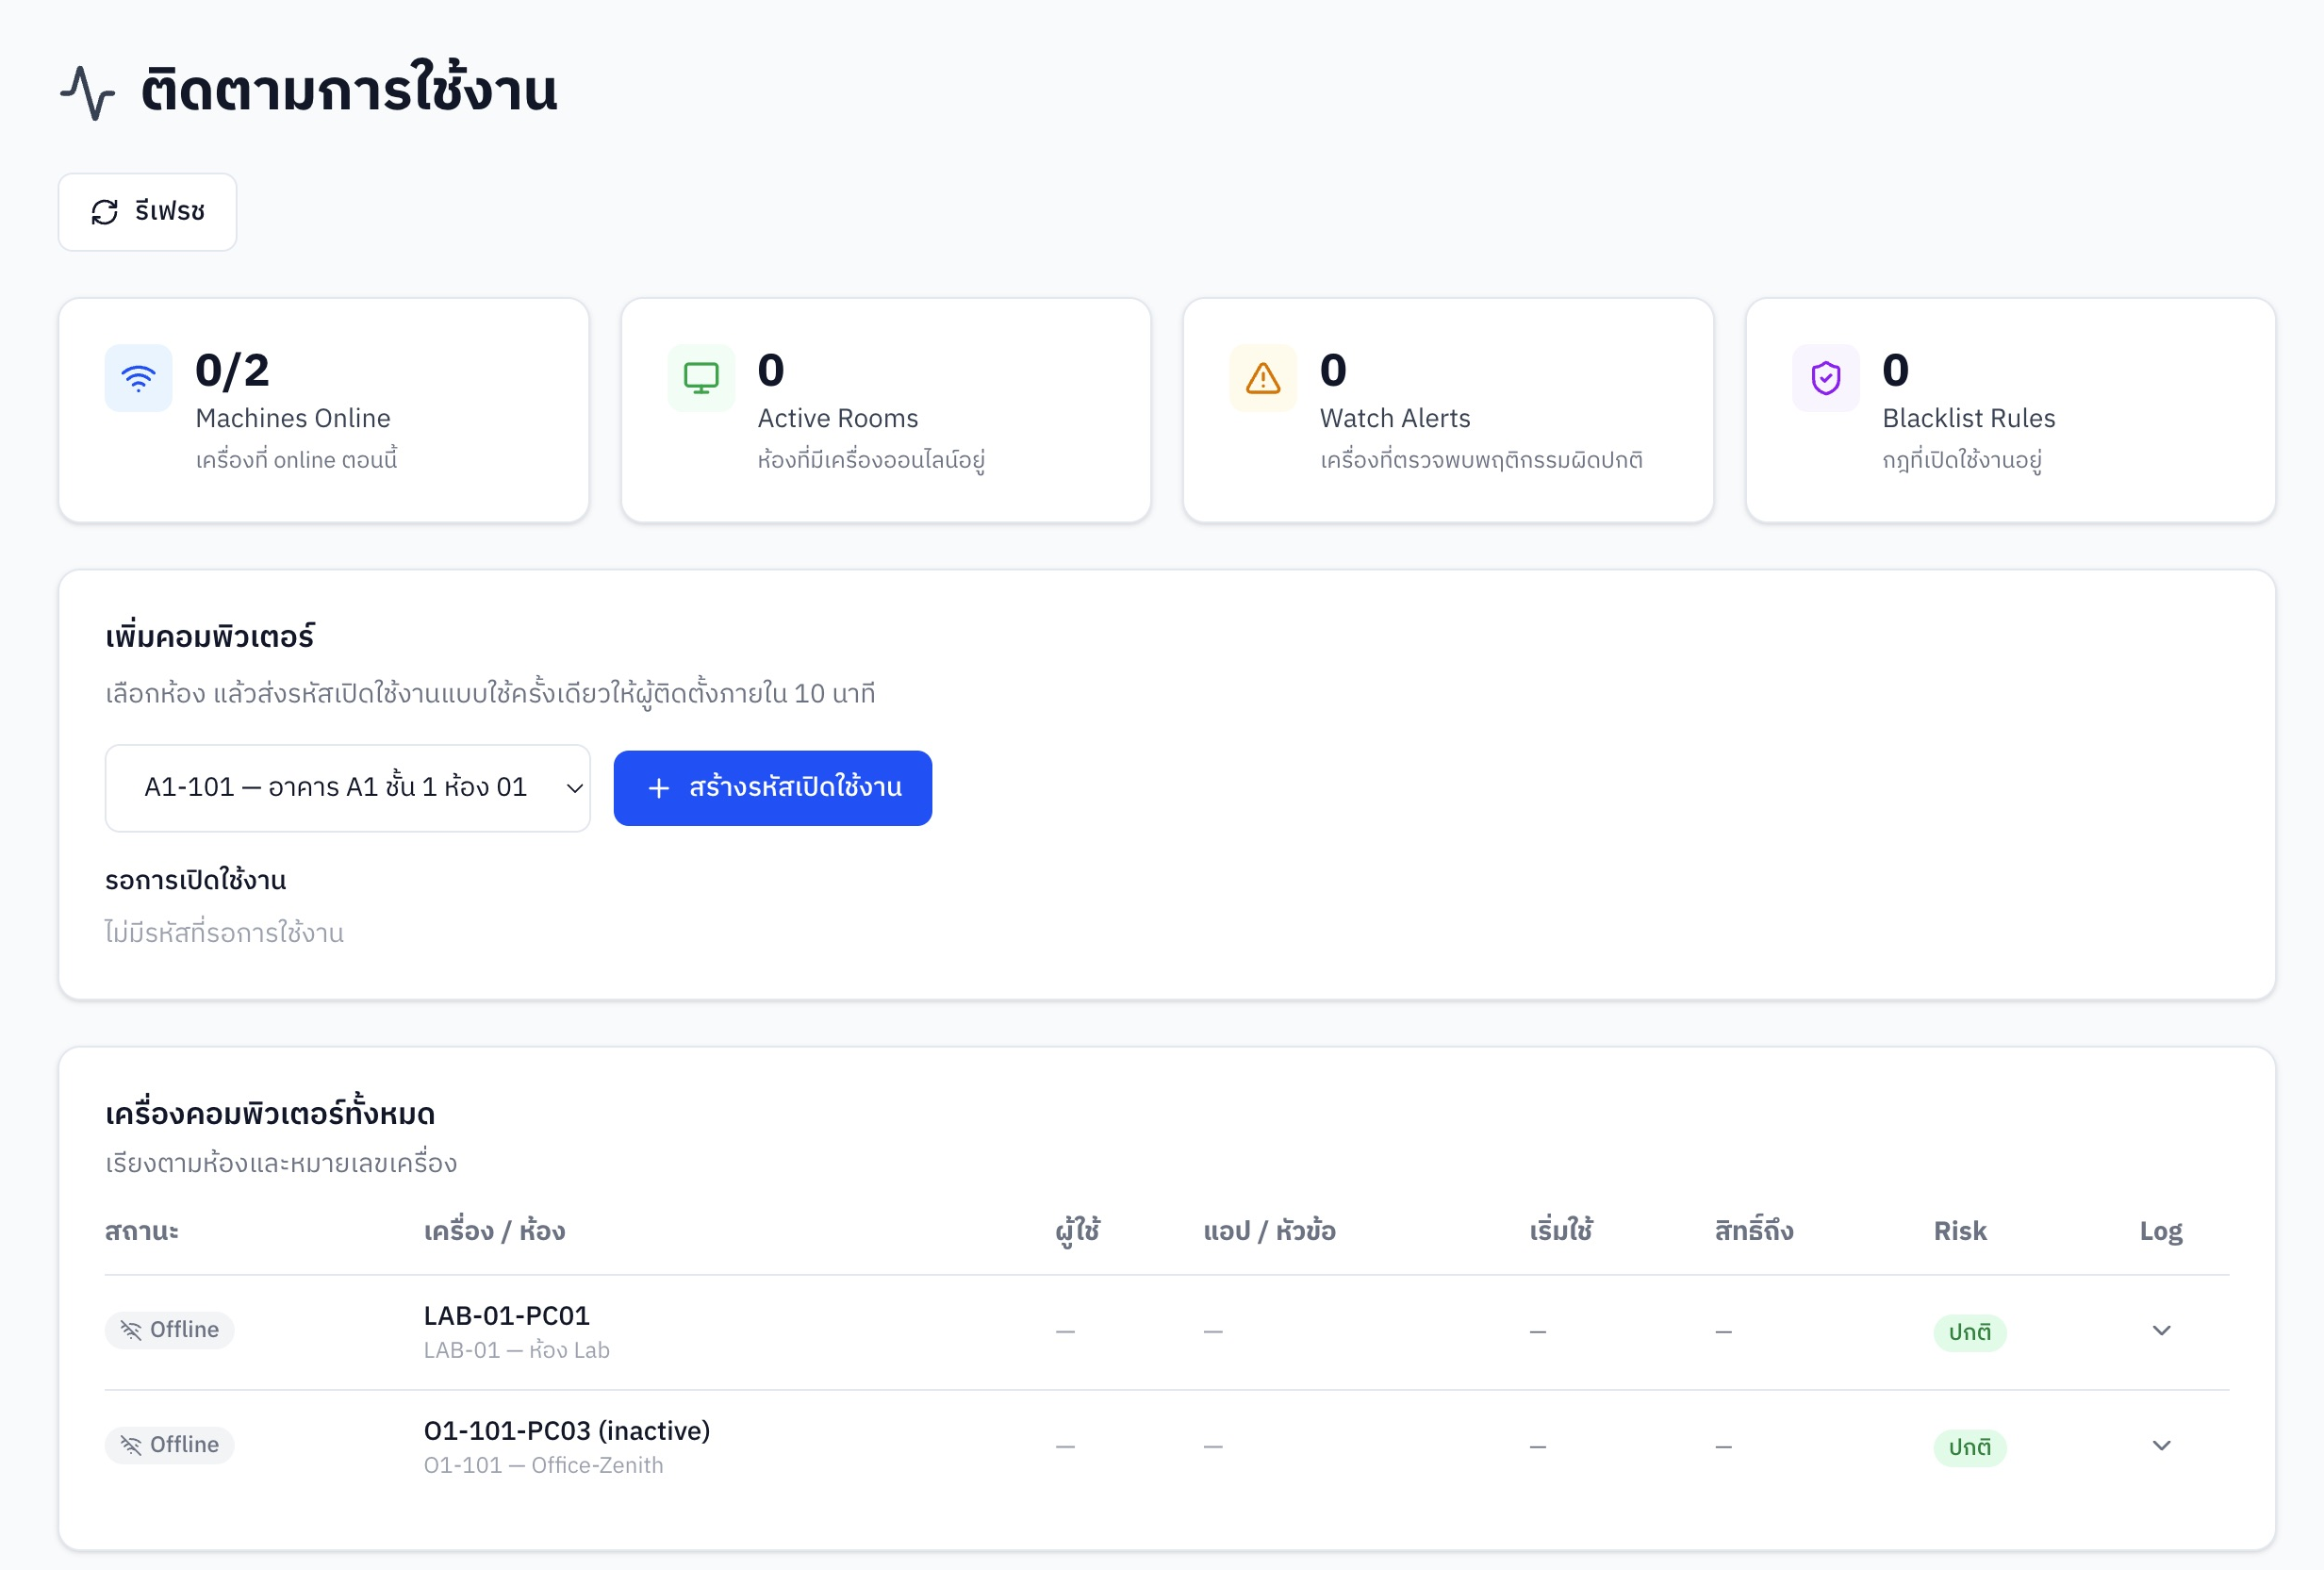
\includegraphics[width=.82\textwidth]{report-assets/ui-tracking-crop.png}\caption{หน้าติดตามสถานะเครื่องคอมพิวเตอร์}\end{figure}

\section{การตรวจที่จุดเข้าใช้ห้อง}
Gate รองรับช่องทางยืนยันที่ระบบเปิดใช้ เช่น ใบหน้าและ QR เมื่อยืนยันผ่านแล้ว ระบบจะตรวจสิทธิ์ของห้องตามข้อมูลและเวลาปัจจุบัน ผลที่แสดงบนหน้าจอเป็นผลการตัดสินของซอฟต์แวร์
\begin{figure}[htbp]\centering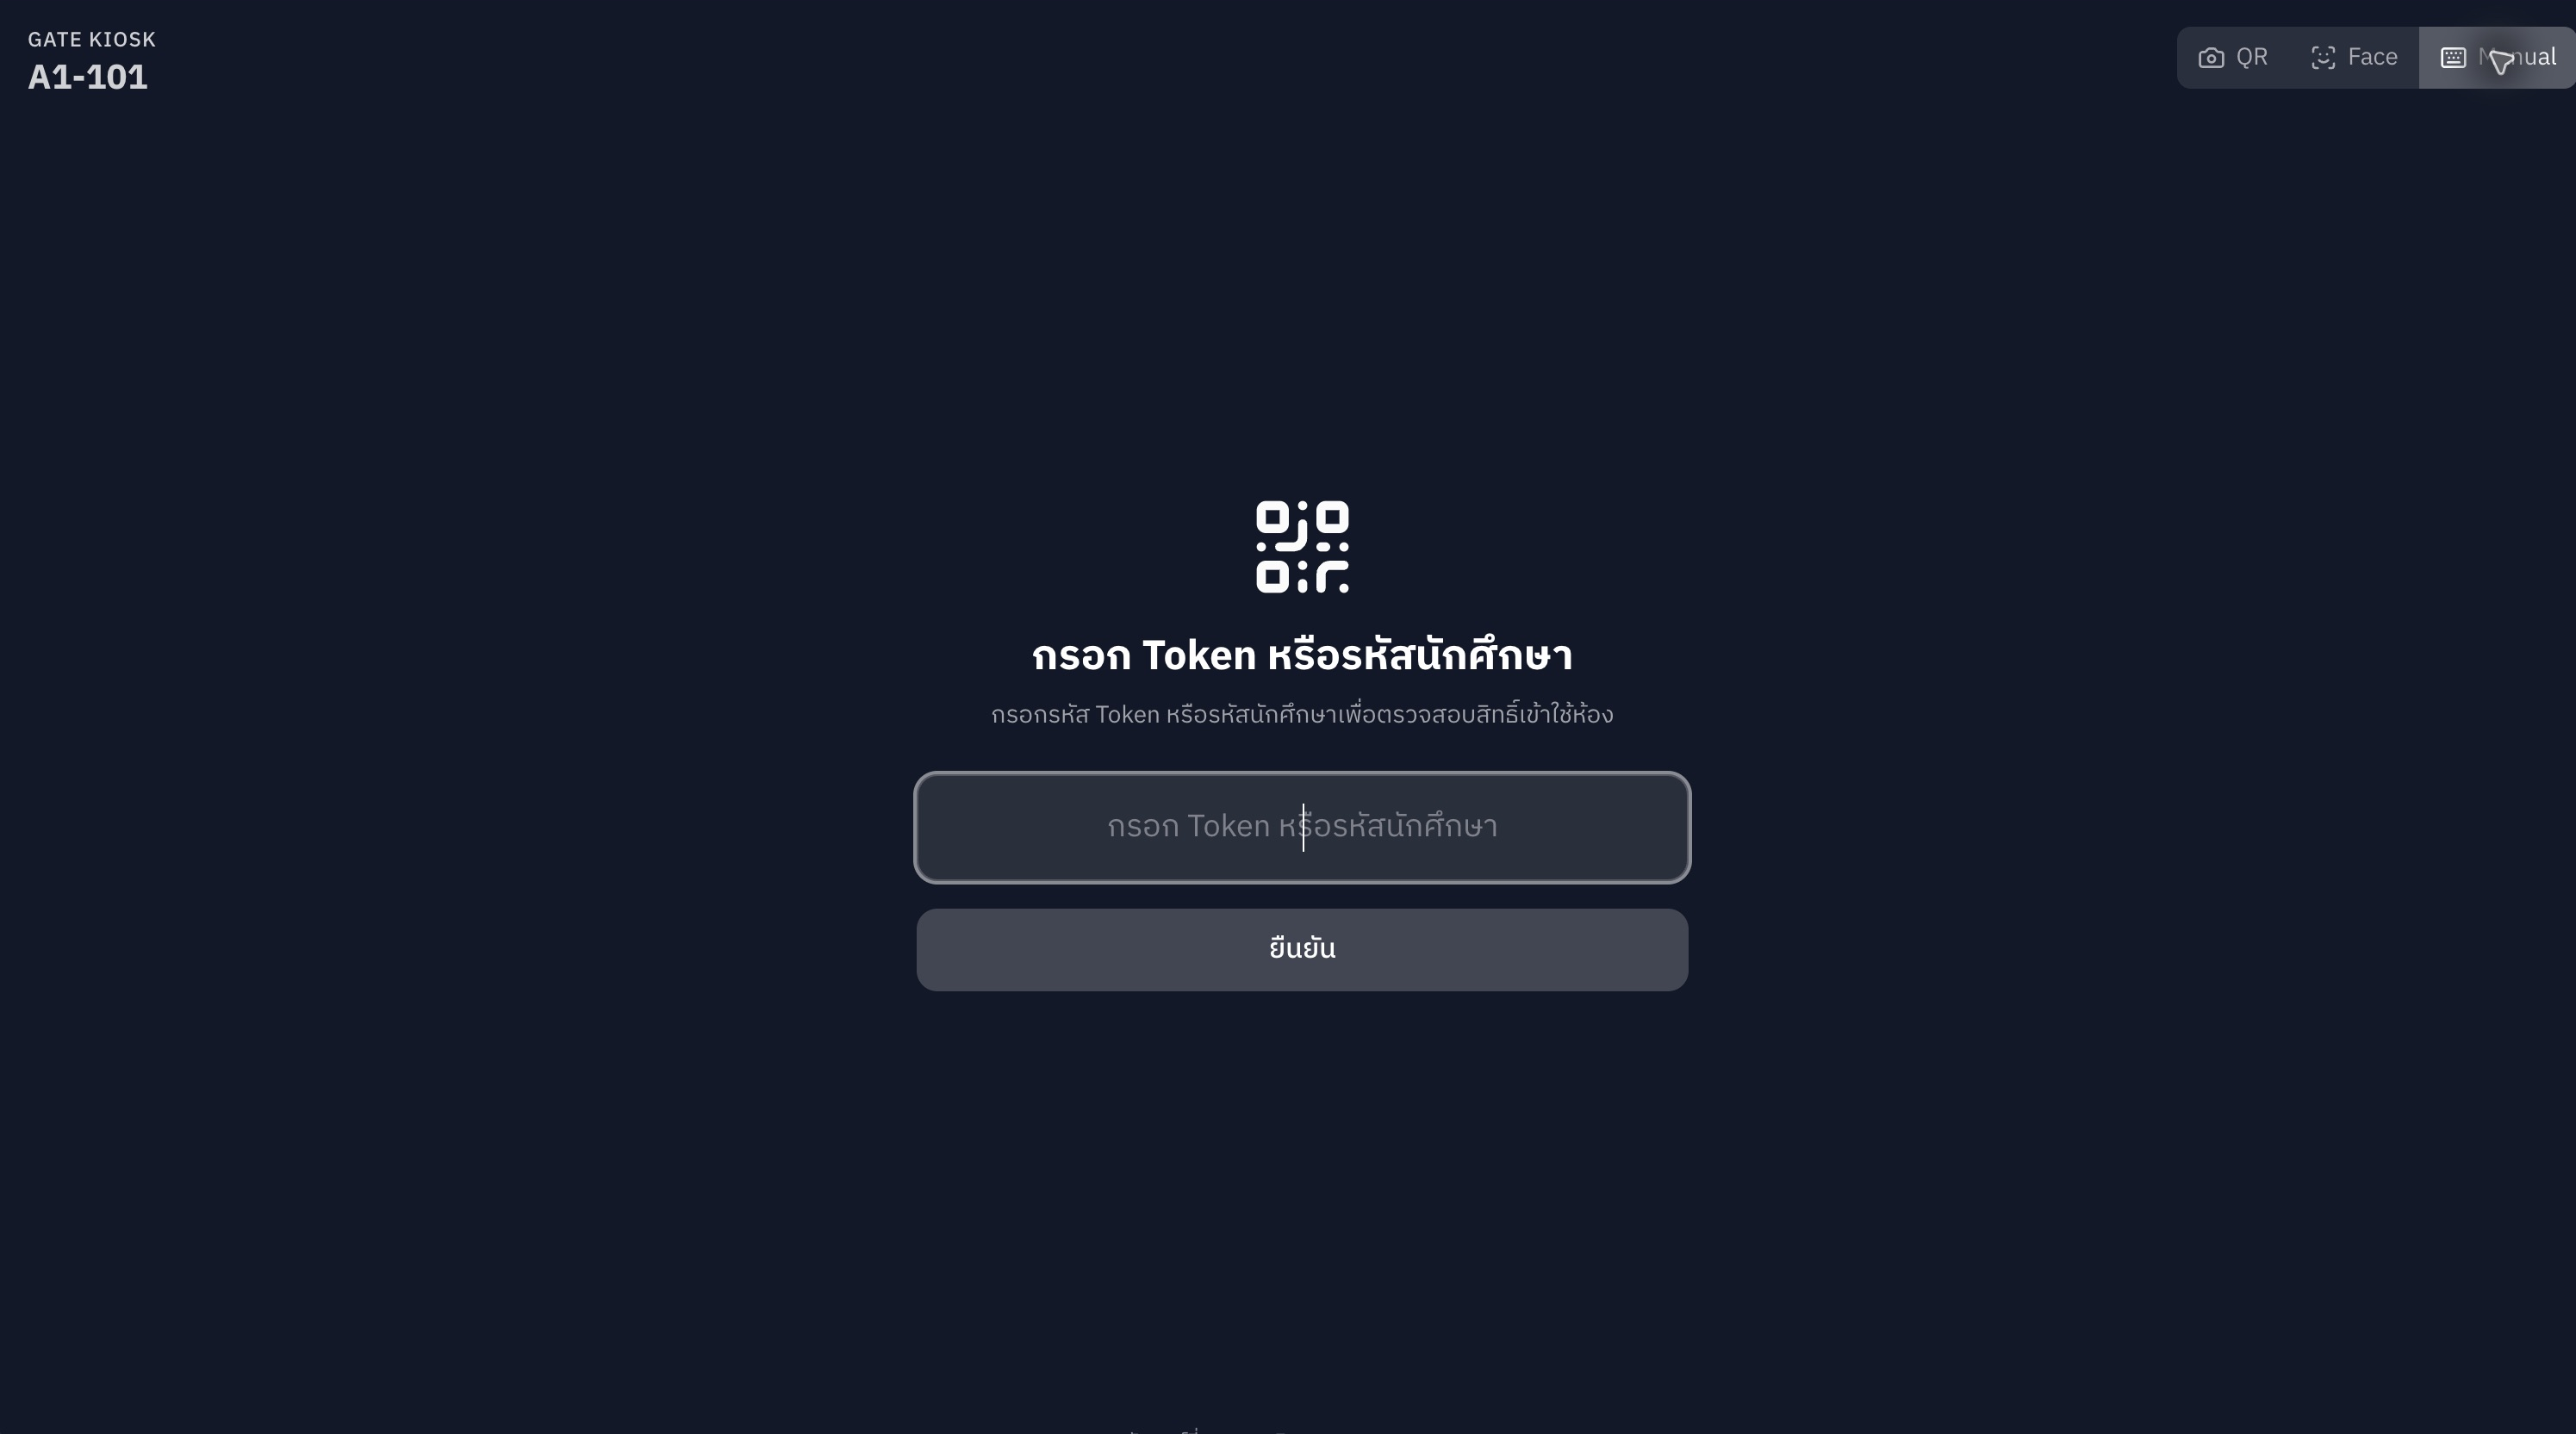
\includegraphics[width=.82\textwidth]{report-assets/ui-gate-crop.png}\caption{หน้าจุดตรวจการเข้าใช้ห้อง}\end{figure}

\section{ผลการทดสอบที่มีหลักฐาน}
วันที่ 20 พฤศจิกายน 2026 รันชุดทดสอบ Vitest ของเว็บโดยไม่รวมการทดสอบฐานข้อมูล ผลคือ 25 ไฟล์ผ่านและ 549 กรณีผ่านทั้งหมด ตารางต่อไปสรุปชิ้นงานและหลักฐานที่ใช้ประกอบการตรวจ

\begin{longtable}{L{51mm}L{45mm}L{42mm}}\caption{สรุปชิ้นงานและหลักฐานการตรวจสอบ}\\\toprule รายการ & หลักฐาน & ผล\\\midrule\endfirsthead
\toprule รายการ & หลักฐาน & ผล\\\midrule\endhead
Web unit tests & Vitest 25 files, 549 tests & ผ่านทั้งหมด\\
เว็บและฐานข้อมูล & ซอร์สโค้ด Prisma schema และ migration & มีองค์ประกอบสำหรับติดตั้ง\\
Face AI & ซอร์สโค้ด FastAPI และหน้า Gate & มีบริการและขั้นตอนยืนยัน\\
Tracking Agent & แพ็กเกจและคู่มือรายระบบ & มีไฟล์ Windows macOS Ubuntu\\
การติดตั้ง Agent macOS & บันทึกการทดลองในคู่มือรุ่น 0.5.0 & ผู้ใช้รายงานว่าเครื่อง Online ได้\\\bottomrule\end{longtable}

\chapter{สรุปผลการดำเนินงาน}
\section{สรุปผลการดำเนินงาน}
โครงงาน Elegant Solution พัฒนาระบบบริหารจัดการห้องปฏิบัติการที่เชื่อมข้อมูลผู้ใช้ ห้อง ตารางเรียน การจอง และสิทธิ์เข้าใช้ไว้ในเว็บแอปพลิเคชันเดียวกัน ระบบกำหนดบทบาท Guest, Student, Admin และ Super Admin เพื่อให้แต่ละกลุ่มเห็นข้อมูลและทำรายการตามหน้าที่ นักศึกษาสามารถตรวจตารางเรียน ค้นหาห้องตามเงื่อนไข และส่งคำขอจอง ส่วนผู้ดูแลสามารถจัดการห้อง กำหนดนโยบายการจอง พิจารณาคำขอ และตรวจข้อมูลการใช้งาน

ส่วนสำคัญของระบบคือการเชื่อมคำขอใช้ห้องกับการตรวจสิทธิ์ในเวลาที่ใช้งานจริง การตัดสินสิทธิ์ใช้ข้อมูลผู้ใช้ ห้อง และช่วงเวลาร่วมกัน โดยพิจารณาตารางเรียนและการจองที่อนุมัติแล้ว รวมถึงรายชื่อผู้ร่วมจองที่บันทึกไว้ในคำขอ จุดตรวจหน้าห้องรองรับการยืนยันด้วยใบหน้าและ QR ตามช่องทางที่เปิดใช้ และบันทึกผลที่เกี่ยวข้องในระบบ วิธีนี้ทำให้ขั้นตอนการค้นหาห้อง การจอง และการตรวจเข้าใช้สัมพันธ์กับข้อมูลชุดเดียวกัน

โครงงานยังพัฒนาบริการ Face AI สำหรับการลงทะเบียนและเปรียบเทียบใบหน้า และ Tracking Agent สำหรับเครื่องคอมพิวเตอร์ห้องปฏิบัติการ Agent ส่งสถานะเครื่องให้ผู้ดูแลเห็นได้แม้ยังไม่มีผู้ใช้เข้าสู่ Agent session ส่วนข้อมูลกิจกรรมผู้ใช้สัมพันธ์กับ session ที่ได้รับสิทธิ์ การแยกสถานะเครื่องออกจากสถานะผู้ใช้ช่วยให้หน้าติดตามแสดงข้อมูลได้ตรงกับเหตุการณ์ที่เกิดขึ้น

การตรวจสอบในสภาพแวดล้อมพัฒนาที่บันทึกไว้เมื่อวันที่ 20 พฤศจิกายน 2026 พบว่าชุดทดสอบเว็บแบบไม่ใช้ฐานข้อมูลผ่าน 549 กรณีจาก 25 ไฟล์ นอกจากนี้ยังมีซอร์สโค้ด โครงสร้างฐานข้อมูล คู่มือติดตั้ง และแพ็กเกจ Agent สำหรับระบบปฏิบัติการที่กำหนด ผลงานจึงครอบคลุมทั้งส่วนที่ผู้ใช้เห็นบนเว็บและส่วนสนับสนุนการทำงานหลังบ้าน โดยการทดสอบบนเครื่องจริงแต่ละระบบปฏิบัติการเป็นขั้นตอนตรวจรับเพิ่มเติมก่อนนำไปใช้งานในพื้นที่จริง

\section{ข้อจำกัดและแนวทางพัฒนา}
การยืนยันใบหน้าในรุ่นปัจจุบันยังไม่ยืนยันการมีชีวิตของผู้ใช้จริง และยังต้องกำหนดนโยบายข้อมูลชีวมิติก่อนใช้ในวงกว้าง การติดตั้ง Agent บน Windows และ Ubuntu ต้องทดสอบบนเครื่องจริงครบขั้นตอน รวมถึง login, activity, logout และ reboot ส่วนการเชื่อมต่ออุปกรณ์เปิดประตูเป็นงานต่อยอดที่ต้องออกแบบและทดสอบแยก

\section{ข้อเสนอแนะ}
ก่อนส่งมอบใช้งานจริง ควรทดลอง flow จากการสร้างบัญชีจนถึงการเข้าใช้ห้องและเครื่องคอมพิวเตอร์ด้วยบัญชีทดสอบที่มีสิทธิ์ถูกต้อง บันทึกผลและภาพหลักฐานแยกตามแพลตฟอร์ม พร้อมตรวจการจัดการข้อมูลส่วนบุคคลและการเข้าถึง log ตามบทบาท

\begin{thebibliography}{9}
\bibitem{next} Next.js. (2026). \textit{Next.js documentation: App Router}. \url{https://nextjs.org/docs/app}
\bibitem{prisma} Prisma. (2026). \textit{Models: Prisma ORM v7}. \url{https://www.prisma.io/docs/orm/v7/prisma-schema/data-model/models}
\bibitem{insightface} InsightFace. (2026). \textit{Model zoo}. \url{https://github.com/deepinsight/insightface/blob/master/model_zoo/README.md}
\bibitem{project} คณะผู้จัดทำโครงงาน. (2026). \textit{Elegant Solution source code and complete manual version 0.5.0}. เอกสารภายในโครงงาน.
\end{thebibliography}

\appendix
\renewcommand{\appendixname}{ภาคผนวก}
\chapter{ไฟล์ประกอบการติดตั้ง}
ซอร์สโค้ดส่วนเว็บอยู่ในโฟลเดอร์ web บริการ AI อยู่ใน ai-service Tracking Agent อยู่ใน agent ฐานข้อมูลและ migration อยู่ใน web/prisma คู่มือการใช้งานและติดตั้งอยู่ใน docs/manual และไฟล์การติดตั้งบนเครื่องใหม่อธิบายไว้ใน docs/PILOT\_DEPLOYMENT.md
\chapter{กรณีทดสอบที่ควรใช้ประกอบการสาธิต}
ตัวอย่างขั้นตอนตรวจรับ: (1) นักศึกษาเข้าสู่ระบบและตรวจตารางเรียน (2) ค้นหาห้องว่างและสร้างการจอง (3) ผู้ดูแลอนุมัติคำขอเมื่อห้องใช้นโยบายอนุมัติด้วยตนเอง (4) ผู้ใช้ยืนยันที่ Gate ในช่วงเวลาที่มีสิทธิ์ (5) Agent ของเครื่องที่จับคู่แล้วแสดงสถานะ Online (6) ผู้ใช้เข้าสู่ Agent session และตรวจ activity เฉพาะช่วงที่ login รายการเหล่านี้เป็นแผนตรวจรับ ไม่ใช่ผลทดสอบจริงทั้งหมด
\end{document}
